% =====================================================================
%  FraudLens - Spark execution workflow
%  Compile:  pdflatex spark_workflow.tex
%  PNG    :  pdftoppm -r 400 -png spark_workflow.pdf spark_workflow
% =====================================================================
\documentclass[border=6pt]{standalone}

\usepackage[T1]{fontenc}
\usepackage{amsmath}
\usepackage{tikz}
\usetikzlibrary{arrows.meta, positioning, calc}
\hyphenpenalty=10000 \exhyphenpenalty=10000

\definecolor{hiFill}{HTML}{E6E6F7}
\definecolor{hiLine}{HTML}{2A2A8C}
\definecolor{inkCol}{HTML}{111111}

\begin{document}
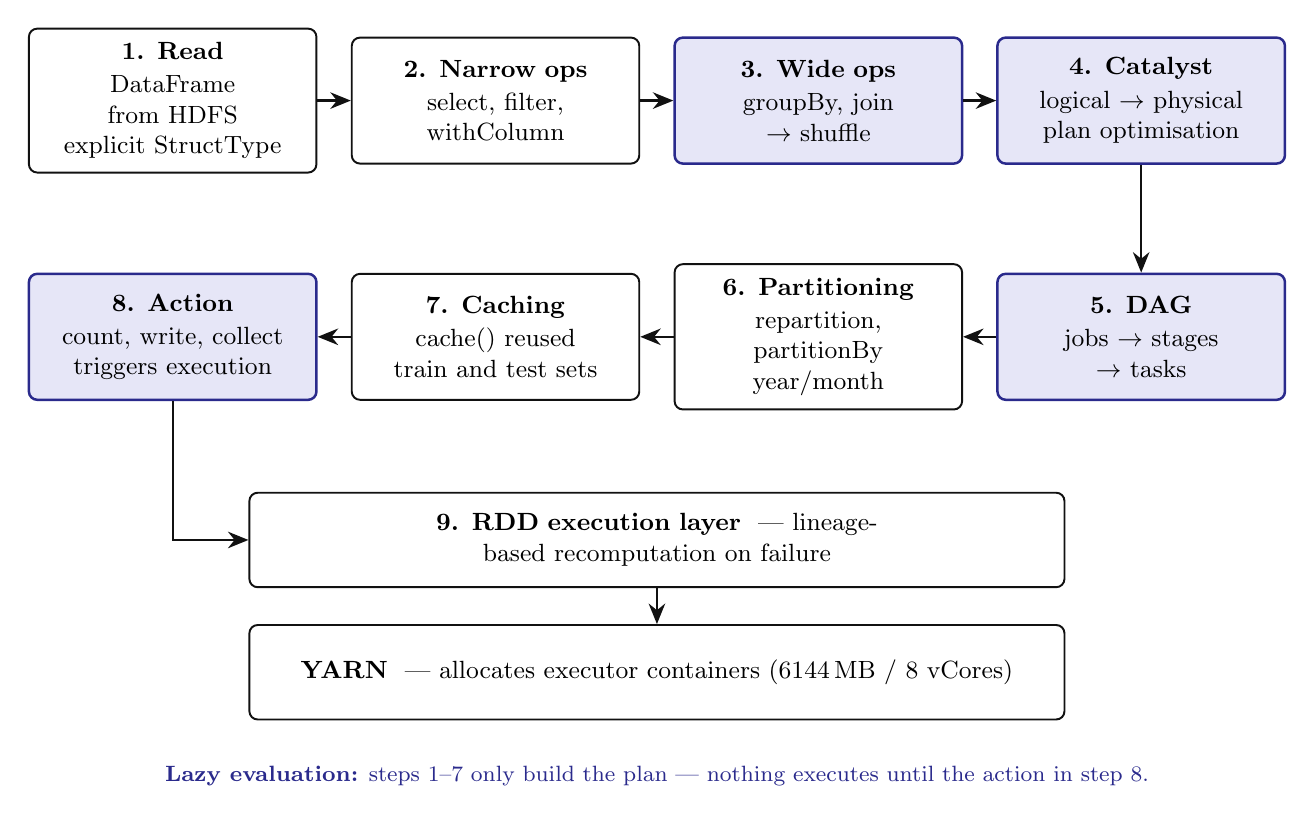
\begin{tikzpicture}[
  font=\small,
  blk/.style={
    draw=inkCol, line width=0.7pt, rounded corners=3pt,
    fill=white, align=center, inner sep=5pt,
    text width=33mm, minimum height=16mm
  },
  hblk/.style={blk, draw=hiLine, line width=0.9pt, fill=hiFill},
  ar/.style={-{Stealth[length=2.6mm,width=2.1mm]}, line width=0.8pt, inkCol}
]

\def\cx{41mm}
\def\ry{30mm}

% ---------------- ROW 1 : left to right -----------------------------
\node[blk]  (s1) at (0*\cx, 0) {\textbf{1. Read}\\[1pt]DataFrame from HDFS\\explicit StructType};
\node[blk]  (s2) at (1*\cx, 0) {\textbf{2. Narrow ops}\\[1pt]select, filter,\\withColumn};
\node[hblk] (s3) at (2*\cx, 0) {\textbf{3. Wide ops}\\[1pt]groupBy, join\\$\rightarrow$ shuffle};
\node[hblk] (s4) at (3*\cx, 0) {\textbf{4. Catalyst}\\[1pt]logical $\rightarrow$ physical\\plan optimisation};

% ---------------- ROW 2 : right to left -----------------------------
\node[hblk] (s5) at (3*\cx, -\ry) {\textbf{5. DAG}\\[1pt]jobs $\rightarrow$ stages\\$\rightarrow$ tasks};
\node[blk]  (s6) at (2*\cx, -\ry) {\textbf{6. Partitioning}\\[1pt]repartition,\\partitionBy year/month};
\node[blk]  (s7) at (1*\cx, -\ry) {\textbf{7. Caching}\\[1pt]cache() reused\\train and test sets};
\node[hblk] (s8) at (0*\cx, -\ry) {\textbf{8. Action}\\[1pt]count, write, collect\\triggers execution};

\draw[ar] (s1) -- (s2);
\draw[ar] (s2) -- (s3);
\draw[ar] (s3) -- (s4);
\draw[ar] (s4) -- (s5);
\draw[ar] (s5) -- (s6);
\draw[ar] (s6) -- (s7);
\draw[ar] (s7) -- (s8);

% ---------------- execution layer -----------------------------------
\node[blk, text width=100mm, minimum height=12mm] (rdd) at (1.5*\cx, -1.86*\ry)
  {\textbf{9. RDD execution layer} \ \textemdash\ lineage-based recomputation on failure};

\node[blk, text width=100mm, minimum height=12mm] (yarn) at (1.5*\cx, -2.42*\ry)
  {\textbf{YARN} \ \textemdash\ allocates executor containers (6144\,MB / 8 vCores)};

\draw[ar] (s8.south) |- (rdd.west);
\draw[ar] (rdd) -- (yarn);

% ---------------- lazy-evaluation note ------------------------------
\node[align=center, font=\footnotesize, text=hiLine]
  at ($(yarn.south)+(0mm,-7mm)$)
  {\textbf{Lazy evaluation:} steps 1--7 only build the plan \textemdash\ nothing executes until the action in step 8.};

\end{tikzpicture}
\end{document}
